%!TEX root = paper.tex

\section{BRATS challenge: framework details}

\subsection{Training dataset (BRATS 2015)}

The BRATS 2015 dataset was available to participants of the challenge. 
It contains $274$ images together with their ground truth annotations. 
One of the interesting aspects of the dataset is the nature of ground truth annotations: $30$ images 
(from the BRATS 2013 dataset) were manually annotated and the remaining were annotated using a consensus of 
segmentation algorithms~\cite{menze2015multimodal}. 
While the ground truth is often of good quality, we note with interest that the consensus of algorithms generally fails at correctly labelling post-resection cavities as in Fig.~\ref{fig:post-resection-cavities} (bottom row). This is likely due to the fact that there is only \textit{one} such training example in the original BRATS 2013 dataset (Fig. \ref{fig:post-resection-cavities}, top row). 

\begin{figure}
\centering
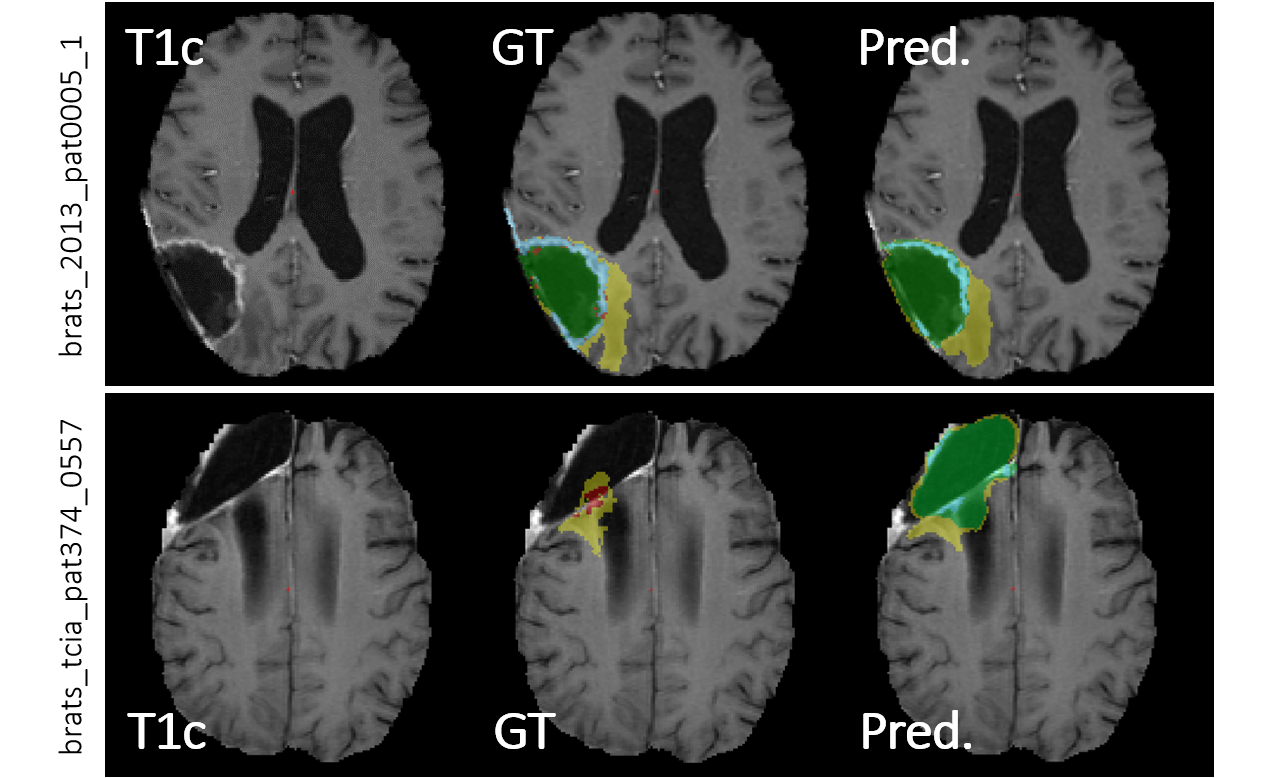
\includegraphics[width=1\textwidth]{images/BRATS2015_post-resection-cavities.png}
\caption{Example images with resection cavities in the BRATS 2015 training set. The first column displays the gadolinium enhanced images, while the second and third respectively display the ground truth annotations and algorithm predictions. Top row: manual annotation. Bottom row: consensus annotation.}
\label{fig:post-resection-cavities}
\end{figure}

We paid particular attention to such training examples. For these cases, we favoured a qualitative, visual 
assessment of correctness over quantitative metrics (DICE overlap or Hausdorff distance) when tuning our pipeline. 
These cases and similar observations motivate the two following choices: 1) An unsupervised SMM/MRF (see below) is trained on the $30$ manually annotated BRATS 2013 images, to initialize the segmentation pipeline. For the background class, SMM weights are spatially varying, so that the model proves reasonably effective to disambiguate potential post-resection cavities from, say, ventricles, and 2) $70$ images from the BRATS 2015 dataset ground truth with high quality annotations are chosen and used for training of the final model. While leading to a slight decrease in quantitative performance of the algorithm, it also qualitatively somewhat improves segmentation results (Fig. \ref{fig:post-resection-cavities}, last column). The same qualitative observations are made on the BRATS 2016 test set. 

\subsection{Pipeline, model and parameter settings}

\noindent
\textbf{Preprocessing.} Image masks are defined from the FLAIR modality, masking out $0$-intensity voxels. The intensity range is standardized: the distribution of voxel intensities within the mask is normalized to a common median and mean absolute error by affine remapping. As a mostly implementation specific step, we further window intensity values to make threshold quantization easier when training DFs: intensities are thresholded and brought within a byte range.\\

\noindent
\textbf{Initialization: SMM/MRF.} An SMM-MRF layer is used to locate the region of interest (ROI) for the whole tumor. The likelihood for each of the five mutually exclusive ground truth classes is modelled using a Student Mixture (SMM) with spatially varying (BG) or fixed (other classes) proportions~\cite{archambeau2007robust}, as a suitably modified variant of~\cite{cordier2015patch}. An MRF prior is assumed over BG, ED and TC. The model is similar in spirit to~\cite{zhang2001segmentation,menze2010generative}. The model is purely unsupervised: we do not use white/grey matter and cerebro-spinal fluid labels in the current implementation, but the resulting components for the background SMM are highly correlated to those labels. %We assume another MRF prior over voxel assignments to the background SMM components, encoding the rough intuition that WM/GM/CSF should smoothly vary spatially. 
Variational Bayesian inference is used at training and test time. Both MRFs define fully connected cliques over the image, with Gaussian decay of pairwise potentials w.r.t. the distance of voxel centers. For this choice of potentials, the dependencies induced by MRF priors in variational updates can be efficiently computed via Gaussian filtering. Inference over $3D$ volumes is fast both at training (seconds or minutes) and test time (seconds).\\

\noindent
\textbf{Auto-context architecture.} $9$ layers of binary DFs are cascaded, cycling between WT, TC and ET probabilities. All layers use the original, raw image channels. The input of first layers is augmented with probability maps from the upstream SMM/MRF, the subsequent layers use probability maps output by previous layers. In addition, the prior probability ``atlas" maps returned by the spatially-varying background SMM/MRF model are passed to the first layers. Many variants of this architecture were informally tested without a significant effect on accuracy.\\

\noindent
\textbf{ROI refinement.} For computational convenience, subsequent layers are run on ROIs rather than the full image. For instance, the second BG vs. WT binary forest only tests points within the mask provided by the first BG vs. WT forest. Similarly at training time, the second layer is trained on subsets of image voxels within the respective image ROIs output by the first layer. Each layer uses masks obtained as dilated versions of the segmentation masks output by the previous layer (dilated resp. by $15$mm, $10$mm, $5$mm).\\

\noindent
\textbf{Parameter settings.} DFs come with a number of parameters, many of which do not seem to strongly affect the pipeline accuracy after informal experiments. Five feature types are used: intensity in a given channel (respectively, at scale $s$), difference of intensities between the voxel of interest (VOI) at scale $s_1$ and an offset voxel at scale $s_2\!>\! s_1$ in a given channel, median of the intensity difference (respectively, absolute difference) between the VOI at scale $s_1$ and the radius-$r$ icosahedron vertices (scale $s_2\! >\!s_1$) in a given channel. Between $100$ and $200$ candidate features are sampled per node. We use $2$ scales: $1$mm and $2$mm for the first layers, $0.5$mm and $1$mm for the second and final layers. The offset along each direction (or the icosahedron radius) is sampled uniformly between $0$mm and $50$mm. The range of feature responses is quantized using $50$ thresholds. The maximum tree depth is set at $12$, and is seldom reached. The number of decision pathways clusters (section \ref{sec: clustering}) is set to $4$. They are created using the first layer of WT, TC, ET (separately for each classification task). The subsampling rate for data bagging is adjusted based on the desired computation time. At each node, the training voxels from $25$ random images serve as tuning set and similarly $30$ (distinct) random images are used for validation (the remaining images are not used to train the node).

\subsection{Test dataset (BRATS 2016)}

The pipeline described above is fully automated. To our knowledge, the BRATS 2015 training dataset pre-processing includes rigid registration (as well as resampling to a common image geometry), bias field correction and skull stripping~\cite{menze2015multimodal}. The BRATS 2016 test dataset contains a number of unprocessed or partially pre-processed images (cf.~Fig.~\ref{fig: test data}). To cope with that, the pipeline was modified to include rigid registration and resampling, bias field correction~\cite{tustison2009n4itk} and skull stripping as part of a semi-automatic pre-processing step.

\begin{figure}
\centering
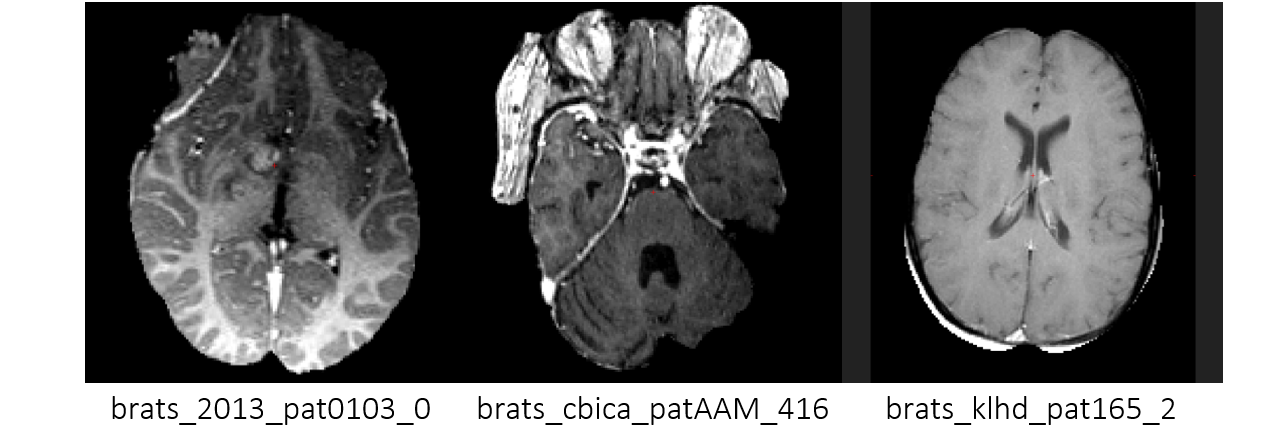
\includegraphics[width=1\textwidth]{images/BRATS2016_example-data.png}
\label{fig: test data}
\caption{BRATS 2016 test data: example of variability not seen in the training set. (Left) Bias field (Middle) Partial skull stripping (Right) Rigid misalignment, different geometry.}
\end{figure}

\section{Results}
\label{sec: results}

The proposed approach is implemented in C\# and F\#. All experiments were performed on a 3.6GHz Intel Xeon processor system with 16GB RAM running Microsoft Windows 10. Training on the BRATS 2015 dataset takes $6$ to $7$ hours (including "testing" on the whole dataset). Testing takes about $20$s per image.

\subsection{BRATS benchmark: Multi-modal MR brain tumor segmentation}

Report running times! Compare to the literature! Try to do the BRATS 2013 leaderboard comparison (array of numbers). BRATS 2015 accuracy vs. number of training images, with varying train/test subsets. Compare to AutoGlioS baseline + to 1-layer CVE forests. Report predicted accuracy (training). Compare to some numbers reported in the literature, point out that our test accuracy was closer.
